\documentclass[12pt]{article}
\usepackage{geometry}
\geometry{a4paper, margin=1in}
\usepackage{setspace}
\usepackage{graphicx}
\usepackage{amsmath, amssymb}
\usepackage{booktabs}
\usepackage{hyperref}
\usepackage{xcolor}

\setstretch{1.1}

\title{\textcolor{blue}{A Design-Based Statistical Investigation into the Determinants of Vehicle Fuel Consumption Efficiency}}
% \large Effects of Cylinders, Horsepower, Weight, and Model Year on Fuel Efficiency:\\ A $2^4$ Factorial Design Using Car Dataset}
\author{Group members: Jiahui Yan, Feng Gu, Ella, Yuzhuo Ye, Taiwo}
\date{}

\begin{document}
\maketitle

\section{Introduction and Research Question}

Fuel efficiency remains one of the most important performance indicators in the automotive industry,
influencing both environmental impact and consumer cost. Previous studies \cite{ahmad2020, greene2017}
have shown \textcolor{blue}{that some mechanical factors}, like engine size and horsepower can affect fuel consumption.

\textcolor{blue}{With the right combination of these factors, improvement on fuel efficiency has been proven achieved,
and it promises the potential for developing more fuel-efficient vehicles by exploring optimal 
configurations on these factors and their interactions.}
Out of this background, this project aims to examine how a series of car factors affect the target variable---fuel efficiency. 

\section{\textcolor{blue}{Research Objectives}}

This project aims to systematically investigate the factors influencing automotive fuel efficiency through
experimental design methodology. The primary objective is to examine how key automotive characteristics individually
and collectively affect miles per gallon (MPG) performance. Specifically, we seek to:
\begin{enumerate}
    \item Determine the main effects of each factor on fuel efficiency
    \item Identify potential interaction effects among these factors to understand how combinations of characteristics influence fuel performance
    \item Apply appropriate statistical analysis including assumption testing and effect size estimation
\end{enumerate}


\section{\textcolor{blue}{Data Description}}
The data are from the Auto MPG Dataset from UCI Machine Learning Repository \cite{uciml2021autompg}.

The Auto MPG Dataset from UCI Machine Learning Repository contains 398 automobiles manufactured between 1970-1982.
The dataset includes nine variables: the dependent variable MPG and eight predictors including cylinders, displacement, horsepower, weight, 
acceleration, model year, origin, and car name,
\footnote{Here the car name is a long string with brand and model information.}
the variable meanings are provided in Table \textcolor{blue}{\ref{tab:dataset_summary}} and their distributions are shown in Figure \textcolor{blue}{\ref{fig:numerical_distributions_with_outliers}}.

\begin{table}[!h]
\centering
\caption{Summary of Variables in the Auto MPG Dataset}
\label{tab:dataset_summary}
\begin{tabular}{p{3cm}p{7cm}p{3cm}}
\toprule
\textbf{Variable} & \textbf{Description} & \textbf{Units / Type} \\
\midrule
mpg\(^*\)(target) & Miles per gallon (fuel efficiency) & $\text{miles}/\text{gallon}$ \\
cylinders & Number of engine cylinders & $\mathbb{N}$ \\
displacement & Engine displacement & $\text{in}^3$(cubic inches) \\
horsepower & Engine power output & $\text{hp}$ \\
weight & Vehicle weight & $\text{lb}$ \\
acceleration & Time to accelerate 0–60 mph & $\text{s}$ \\
model year & Year of manufacture (two-digit) & $\mathbb{N}$ \\
origin & Country/region of origin & $\{1,2,3\}$ \\
car name & Car make and model & $\text{string}$ \\
\bottomrule
\end{tabular}
\end{table}

\begin{figure}[!h]
    \centering
    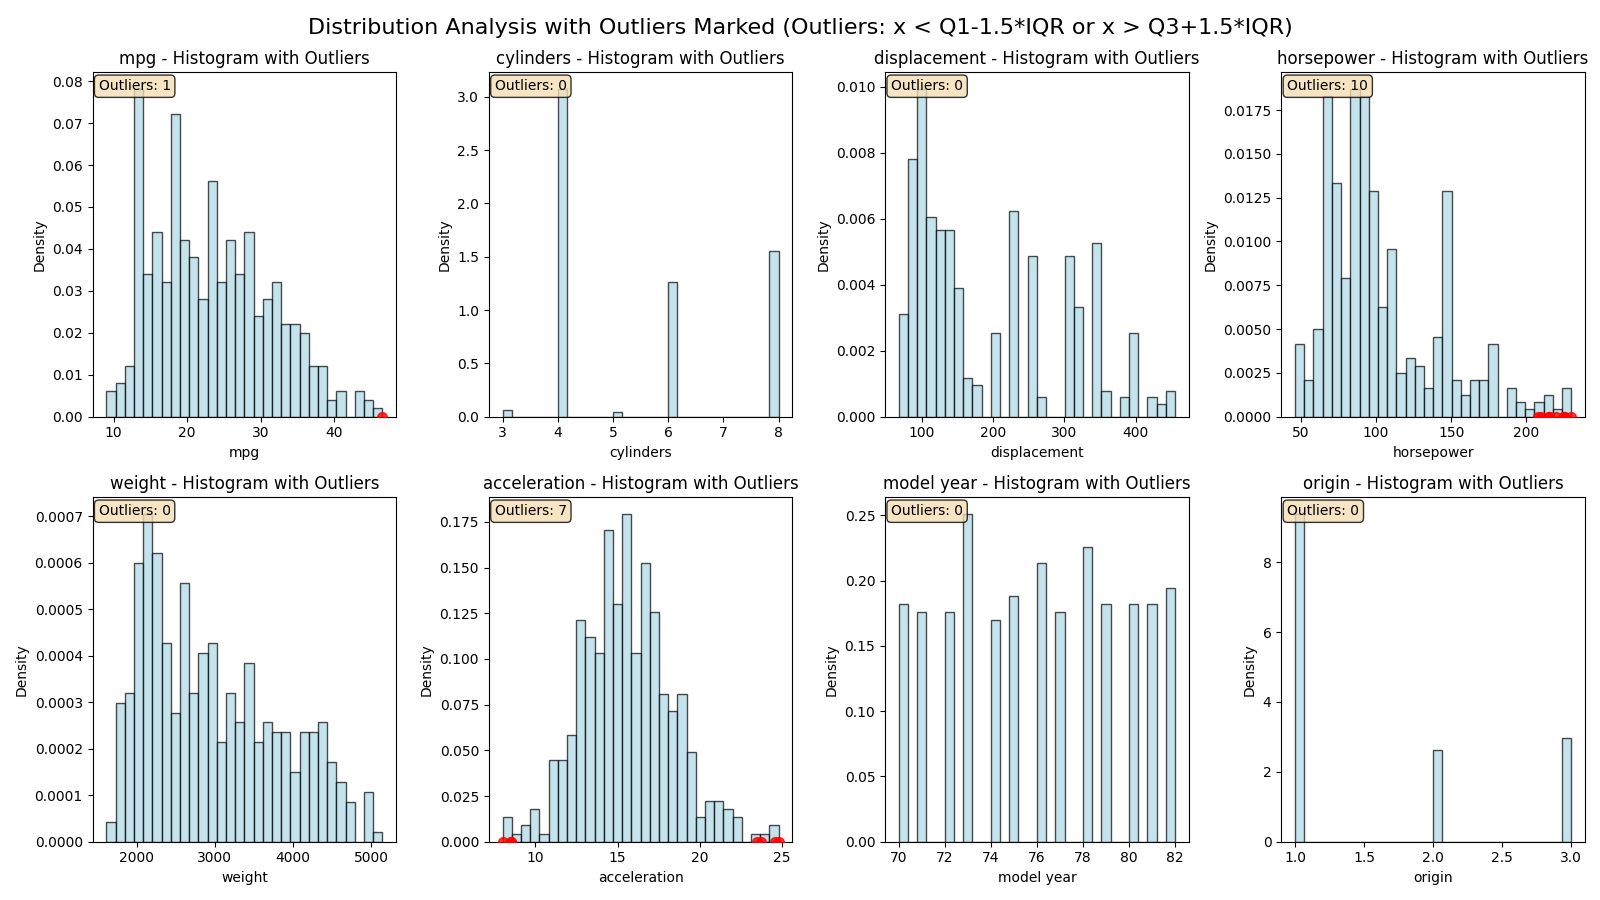
\includegraphics[width=0.8\textwidth]{../results/numerical_distributions_with_outliers.png}
    \caption{Distributions of Numerical Variables in the Auto MPG Dataset}
    \label{fig:numerical_distributions_with_outliers}
\end{figure}



\section{Brief Literature Review}

Studies in automotive engineering and energy policy emphasize that vehicle weight and engine design strongly influence fuel efficiency.

\begin{itemize}
    \item \cite{ahmad2020} found that a 10\% reduction in weight improves fuel economy by up to 8\%.
    \item \cite{greene2017} reported that higher cylinder counts and engine power typically reduce mpg due to increased energy requirements.
    \item \cite{li2022} observed that newer model years integrate improved engine management and aerodynamics, enhancing fuel efficiency despite higher horsepower.
\end{itemize}

While these studies analyzed individual factors, few examined their interaction effects through factorial experiments. This project addresses that gap by using a $2^4$ factorial design to quantify both individual and combined influences of mechanical and temporal factors on mpg.



\clearpage
\section{\textcolor{blue}{Hypotheses and Statistical Models}}

The following hypotheses will be tested to examine the relationships between automotive characteristics and fuel efficiency at $\alpha = 0.05$ significance level:

\subsection{Main Effect Hypotheses}

\begin{table}[h]
\centering
\caption{Main Effect Hypotheses for Automotive Fuel Efficiency Analysis}
\label{tab:main_hypotheses}
\begin{tabular}{p{2.5cm}p{6cm}p{6cm}}
\toprule
\textbf{Variable} & \textbf{Null Hypothesis ($H_0$)} & \textbf{Alternative Hypothesis ($H_1$)} \\
\midrule
Cylinders & Number of cylinders has no significant effect on MPG & Number of cylinders has a significant effect on MPG \\
\midrule
Displacement & Engine displacement has no significant effect on MPG & Engine displacement has a significant effect on MPG \\
\midrule
Horsepower & Engine horsepower has no significant effect on MPG & Engine horsepower has a significant effect on MPG \\
\midrule
Weight & Vehicle weight has no significant effect on MPG & Vehicle weight has a significant effect on MPG \\
\midrule
Acceleration & Acceleration time has no significant effect on MPG & Acceleration time has a significant effect on MPG \\
\midrule
Model Year & Model year has no significant effect on MPG & Model year has a significant effect on MPG \\
\midrule
Origin & Country/region of origin has no significant effect on MPG & Country/region of origin has a significant effect on MPG \\
\bottomrule
\end{tabular}
\end{table}

\subsection{Statistical Model Formulations and Hypotheses for Key Relationships}

\textbf{ANOVA Model for Categorical Factors:}
\begin{align}
\text{MPG}_{ijk} &= \mu + \alpha_i + \beta_j + (\alpha\beta)_{ij} + \epsilon_{ijk}
\end{align}

\noindent where $i$ represents cylinder groups, $j$ represents origin groups, and $(\alpha\beta)_{ij}$ represents interaction effects.
The error term is tentatively assumed to follow \(\epsilon_{ijk} \sim N(0,\sigma^2)\) for observations within each group.

\textbf{Multiple Linear Regression Model:}
\begin{align}
\text{MPG} &= \beta_0 + \beta_1(\text{Cylinders}) + \beta_2(\text{Displacement}) + \beta_3(\text{Horsepower}) \nonumber \\
&\quad + \beta_4(\text{Weight}) + \beta_5(\text{Acceleration}) + \beta_6(\text{Model Year}) \nonumber \\
&\quad + \beta_7(\text{Origin}_2) + \beta_8(\text{Origin}_3) + \epsilon
\end{align}

\noindent where $\epsilon \sim N(0,\sigma^2)$ and Origin is dummy-coded with USA as reference category.

\begin{table}[!h]
\centering
\caption{Specific Directional Hypotheses}
\label{tab:directional_hypotheses}
\begin{tabular}{p{3cm}p{4.5cm}p{7cm}}
\toprule
\textbf{Relationship} & \textbf{Null Hypothesis($H_0$)} & \textbf{Alternative Hypothesis($H_1$)} \\
\midrule
Cylinders-MPG & $\beta_{\text{cylinders}} = 0$ & $\beta_{\text{cylinders}} < 0$ \newline (More cylinders decrease MPG) \\
\midrule
Weight-MPG & $\beta_{\text{weight}} = 0$ & $\beta_{\text{weight}} < 0$ \newline (Higher weight decreases MPG) \\
\midrule
Horsepower-MPG & $\beta_{\text{horsepower}} = 0$ & $\beta_{\text{horsepower}} < 0$ \newline (Higher horsepower decreases MPG) \\
\midrule
Model Year-MPG & $\beta_{\text{year}} = 0$ & $\beta_{\text{year}} > 0$ \newline (Newer cars have higher MPG) \\
\midrule
Origin Effect & $\mu_{\text{USA}} = \mu_{\text{Europe}} = \mu_{\text{Japan}}$ & At least one origin mean differs significantly \\
\bottomrule
\end{tabular}
\end{table}

\clearpage

\section{Overview of Experimental Design}

\subsection{Design Type}

A $2^4$ factorial design (no replication) will be used. This design evaluates four independent factors, each at two levels:

\begin{table}[!h]
\centering
\begin{tabular}{lll}
\toprule
\textbf{Factor} & \textbf{Levels} & \textbf{Type} \\
\midrule
Cylinders & 4 vs. 8 & Discrete \\
Horsepower & Low vs. High (median split) & Continuous (categorized) \\
Weight & Low vs. High (median split) & Continuous (categorized) \\
Model Year & Old vs. New (pre-1980 vs. post-1980) & Categorical \\
\bottomrule
\end{tabular}
\end{table}

Dependent Variable: \textit{Miles per Gallon (mpg)} — continuous measure of fuel efficiency.

\subsection{Experimental Units}

Each car in the dataset represents one experimental unit. Cars are assigned into treatment combinations according to the four factors. With a $2^4$ factorial design, there are 16 treatment combinations (e.g., 4-cylinder, low horsepower, low weight, old model year).

\subsection{Randomization and Control}

\begin{itemize}
    \item \textbf{Randomization:} Cars are randomly selected from the dataset for each treatment combination to minimize selection bias.
    \item \textbf{Control Variables:} Transmission type and engine displacement will be monitored to reduce confounding effects.
\end{itemize}

\section{Statistical Analysis Plan}

\subsection{Data Preparation}

Data from the car dataset will be preprocessed in \textsf{R}:

\begin{itemize}
    \item Handle missing values using mean or median imputation.
    \item Categorize continuous predictors (horsepower and weight) into “low” and “high” based on median splits.
    \item Code categorical variables (e.g., cylinders = \{4, 8\}; model\_year = \{old, new\}).
\end{itemize}

\subsection{Analysis Method}

A four-factor ANOVA ($2^4$ design) will be conducted to test main and interaction effects. 

If assumptions are not met:
\begin{itemize}
    \item Apply transformation (e.g., $\log(\text{mpg})$).
    \item Use multiple regression as an alternative model.
\end{itemize}

\subsection{Statistical Tools}

\begin{itemize}
    \item Normality test: Shapiro–Wilk test
    \item Variance homogeneity: Levene’s test
    \item Effect size: Partial $\eta^2$ using \texttt{effectsize} package
    \item Visualization: Interaction plots and residual diagnostics (\textsf{ggplot2}, \textsf{interactions} packages)
\end{itemize}


\textbf{Main Effects:} Cars with fewer cylinders, lower horsepower, lighter weight, and newer models are expected to have higher mpg.

\textbf{Interaction Effects:}
\begin{itemize}
    \item The negative effect of weight may be stronger for older cars.
    \item The effect of horsepower may depend on the number of cylinders.
\end{itemize}

These outcomes could provide insights into energy-efficient automotive design and environmental sustainability initiatives.




\clearpage

\section{\textcolor{blue}{Preliminary Analysis: One-Way ANOVA on Car Origin and Fuel Efficiency}}

% \subsection{One-Way ANOVA: Effect of Car Origin on Fuel Efficiency}

As a preliminary investigation, we conducted a one-way ANOVA to examine whether car origin (USA, Europe, Japan) 
significantly affects fuel efficiency, and this analysis serves as a foundational step to more complex multi-factor designs.

\textbf{Experimental Design:} The one-way ANOVA employed a completely randomized design with car origin 
as the single factor at three levels: Origin 1 (USA, n=249), Origin 2 (Europe, n=70), and Origin 3 (Japan, n=79). 
Each car represents an independent experimental unit, with MPG as the continuous response variable.

\textbf{Hypotheses Tested:}
\begin{itemize}
    \item $H_0$: $\mu_{\text{USA}} = \mu_{\text{Europe}} = \mu_{\text{Japan}}$ (all origin groups have equal mean MPG)
    \item $H_1$: At least one origin group has a significantly different mean MPG
\end{itemize}


\begin{figure}[!h]
    \centering
    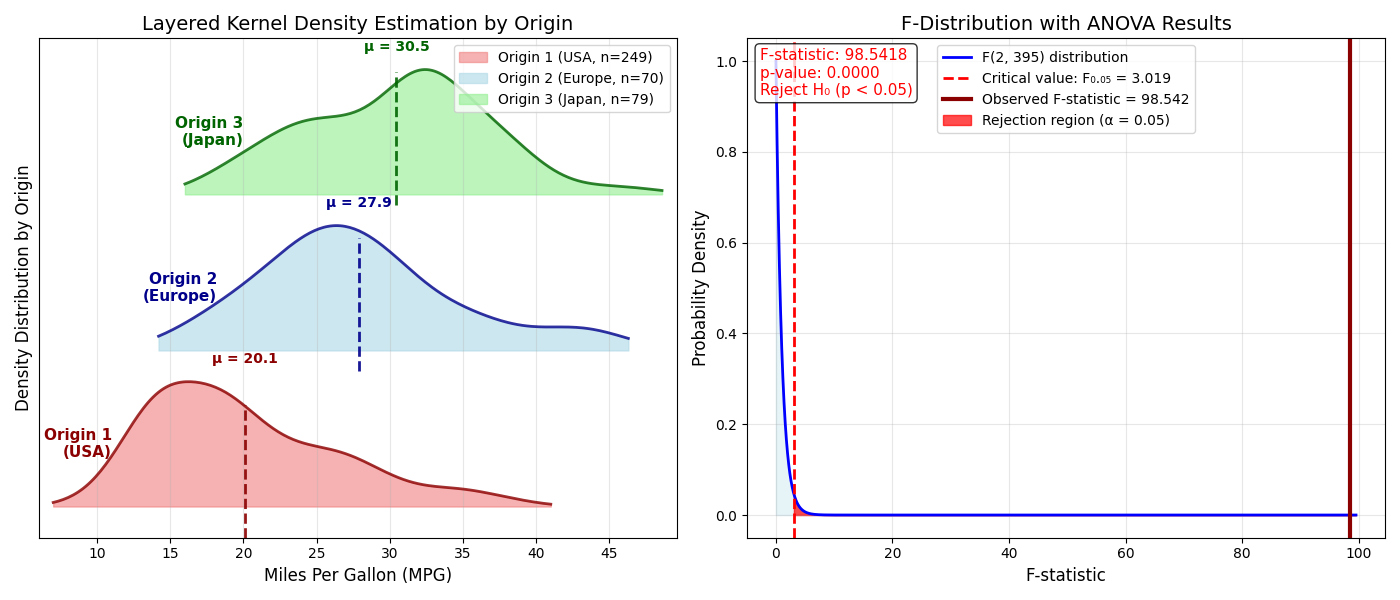
\includegraphics[width=0.9\textwidth]{../results/anova_origin_mpg.png}
    \caption{Preliminary ANOVA Results: Effect of Car Origin on Fuel Efficiency (MPG)}
    \label{fig:preliminary_anova}
\end{figure}



\begin{table}[h!]
\centering
\caption{One-Way ANOVA Results: Effect of Car Origin on Fuel Efficiency (MPG)}
\label{tab:anova_results}
\begin{tabular}{lc}
\toprule
\textbf{ANOVA Summary} & \textbf{Value} \\
\midrule
Null Hypothesis ($H_0$) & All group mpg means are equal \\
Alternative Hypothesis ($H_1$) & At least one group mpg mean differs \\
Significance level ($\alpha$) & 0.050 \\
\midrule
Total sample size ($N$) & 398 \\
Number of groups ($k$) & 3 \\
Degrees of freedom (Between groups) & 2 \\
Degrees of freedom (Within groups) & 395 \\
Critical $F$-value & 3.0186 \\
Observed $F$-statistic & 98.5418 \\
$p$-value & $< 0.001$ \\
\midrule
Statistical Decision & \textbf{Reject $H_0$} \\
Effect Size ($\eta^2$) & 0.3329 \\
\bottomrule
\end{tabular}
\end{table}

The ANOVA revealed a highly significant effect of car origin on fuel efficiency
\((F_{(2,395)} = 98.54\), \(p < 0.001\), $\eta^2$ = 0.333). Japanese cars showed highest efficiency (M = 30.45), 
followed by European (M = 27.89) and American cars (M = 20.08), leading to rejection of the null hypothesis.

This preliminary analysis confirms significant regional differences in automotive fuel efficiency, supporting 
the inclusion of origin as a key factor in subsequent multi-factorial designs.


% ====================================
\clearpage
\section{References}
\begin{thebibliography}{9}

\bibitem{ahmad2020}
Ahmad, N., et al. (2020). \textit{Weight reduction and fuel efficiency in automotive design: An integrated assessment}. Transportation Research Part D: Transport and Environment, 86, 102446.

\bibitem{greene2017}
Greene, D. L., \& Welch, T. (2017). \textit{Impact of engine size and vehicle weight on fuel economy: Policy implications}. Energy Policy, 108, 273–282.

\bibitem{li2022}
Li, F., \& Zhao, J. (2022). \textit{Advances in automotive efficiency: The role of model year innovation}. Applied Energy, 325, 119823.

\bibitem{usdoe2021}
U.S. Department of Energy. (2021). \textit{Fuel Economy Trends Report}. Retrieved from \url{https://www.energy.gov}

\bibitem{uciml2021autompg}
U.S. Department of Energy. (2021). \textit{Auto MPG Dataset}. 
UCI Machine Learning Repository. Retrieved from \url{https://www.kaggle.com/datasets/uciml/autompg-dataset}

\end{thebibliography}

\section{Appendix}

\subsection{Figures}
\begin{figure}[!h]
    \centering
    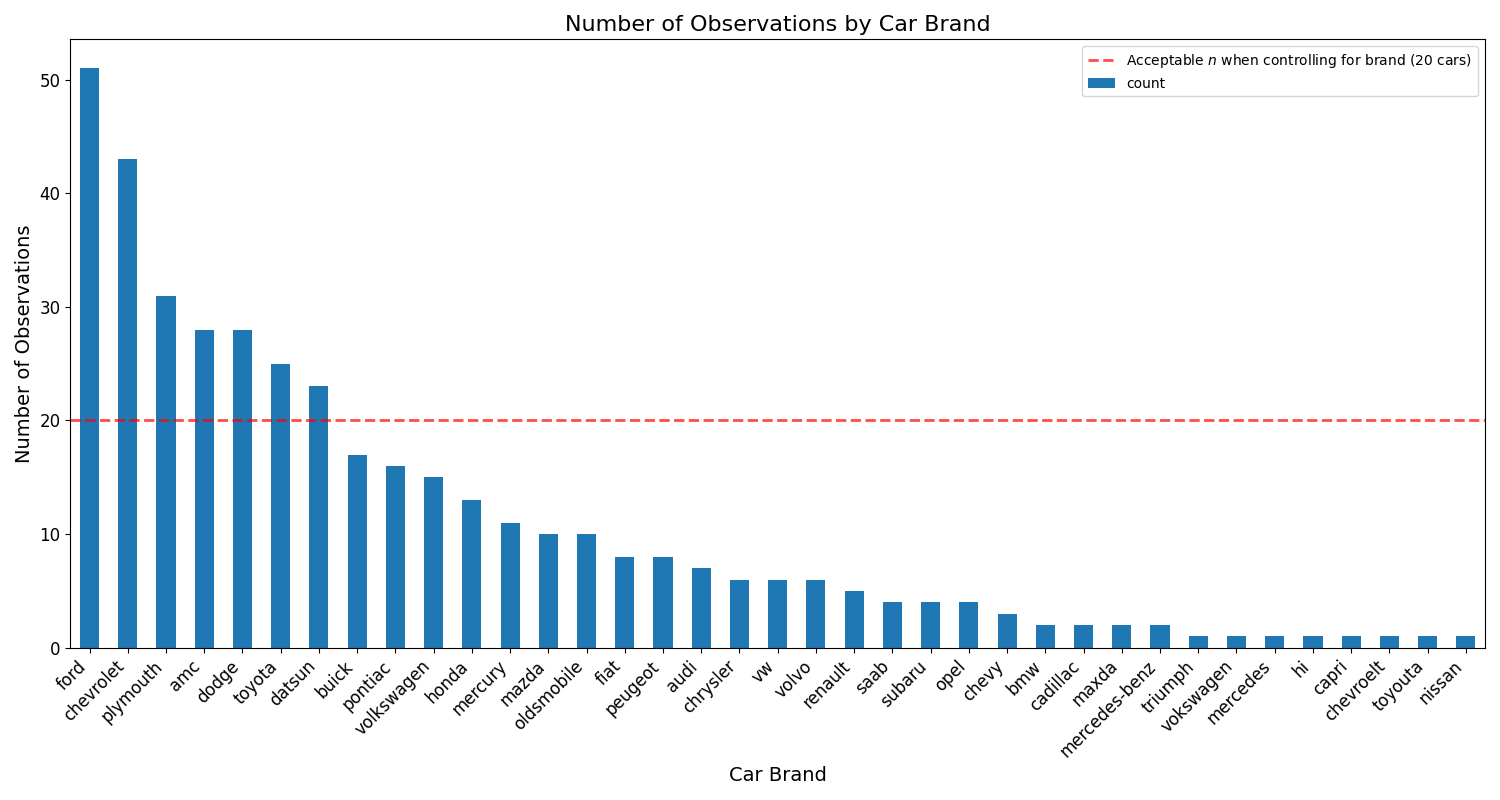
\includegraphics[width=0.8\textwidth]{../results/brand_distribution.png}
    \caption{Distribution of samples by Car Brand}
    \label{fig:brand_distribution}
\end{figure}

\subsection{Tables}

\begin{table}[h!]
\centering
\caption{Descriptive Statistics of Fuel Efficiency (MPG) by Car Origin}
\label{tab:descriptive_stats}
\begin{tabular}{lccc}
\toprule
\textbf{Origin} & \textbf{Sample Size ($n$)} & \textbf{Mean MPG} & \textbf{Standard Deviation} \\
\midrule
Origin 1 (USA) & 249 & 20.08 & 6.40 \\
Origin 2 (Europe) & 70 & 27.89 & 6.72 \\
Origin 3 (Japan) & 79 & 30.45 & 6.09 \\
\midrule
\textbf{Total} & \textbf{398} & \textbf{23.51} & \textbf{7.82} \\
\bottomrule
\end{tabular}
\end{table}

\subsection{Ethical Considerations}

Although the dataset is non-human and publicly available, ethical integrity is maintained by:

\begin{itemize}
    \item \textbf{Data Source:} \url{https://www.kaggle.com/datasets/uciml/autompg-dataset}
    \item \textbf{Privacy and Compliance:} Ensuring no personally identifiable information is used.
    \item \textbf{Reproducibility:} Providing Python code and random seeds for full replication.
    \item \textbf{Fair Representation:} Avoiding selective reporting or p-hacking.
    \item \textbf{Academic Integrity:} Properly citing all sources and acknowledging dataset creators.
\end{itemize}




\end{document}
